\documentclass[tikz]{standalone}
% \usetikzlibrary{trees,calc}
\usepackage{pgfplots}
\pgfplotsset{compat = newest}
\begin{document}

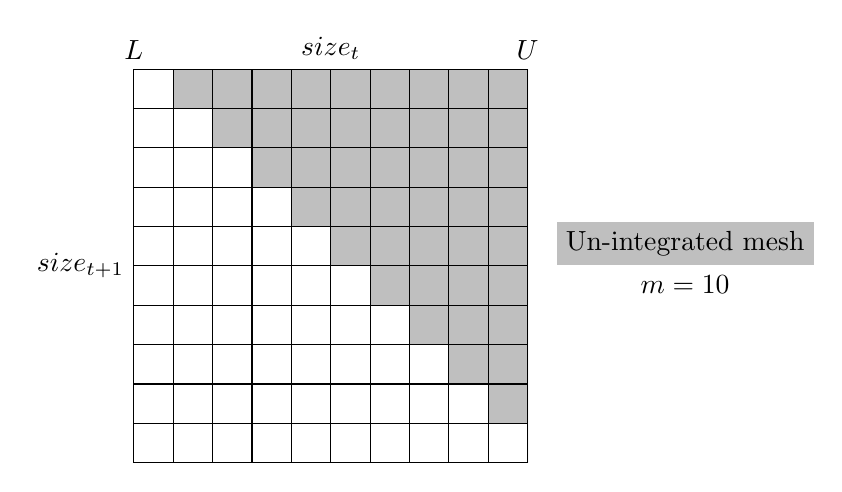
\begin{tikzpicture}
    \foreach \i in {5,4.5,...,0.5}{
            {\fill[gray!50] (\i, 5-\i) -- (5,5-\i) -- (5,5) -- (\i,5);}
    }

    \draw (0,0) grid[step=.5] (5,5);
    \draw (2.5,5) node[above]{$size_t$} ;
    \draw (0,2.5) node[left]{$size_{t+1}$} ;

    \draw(7,2.5) node[fill=gray!50,above] {Un-integrated mesh};
    \draw(7,2.5) node[below] {$m = 10$};
    \draw(0,5) node[above] {$L$};
    \draw(5,5) node[above] {$U$};

\end{tikzpicture}

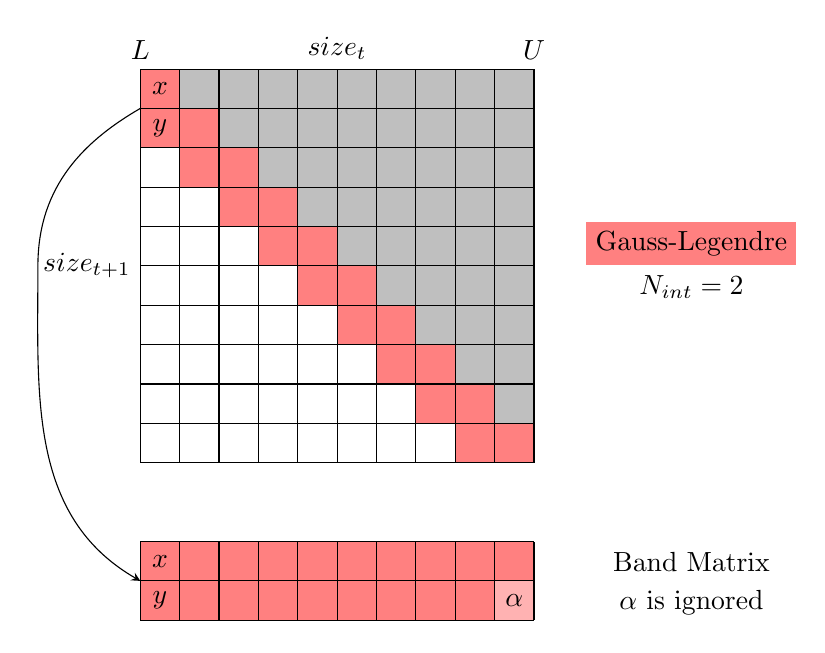
\begin{tikzpicture}
    \foreach \i in {4,3.5,...,0}{
            {\fill[red!50] (\i, 5-\i-1) -- (5,5-\i-1) -- (5,5) -- (\i,5);}
    }
    \foreach \i in {5,4.5,...,0.5}{
            {\fill[gray!50] (\i, 5-\i) -- (5,5-\i) -- (5,5) -- (\i,5);}
    }

    \draw (0,0) grid[step=.5] (5,5);
    \draw (2.5,5) node[above]{$size_t$} ;
    \draw (0,2.5) node[left]{$size_{t+1}$} ;
    \draw(0,5) node[above] {$L$};
    \draw(5,5) node[above] {$U$};

    \draw(7,2.5) node[fill=red!50,above] {Gauss-Legendre};
    \draw(7,2.5) node[below] {$N_{int} = 2$};

    \fill[red!50] (0, -2) -- (5,-2) -- (5, -1) -- (0,-1);
    \fill[red!30] (4.5, -2) -- (4.5,-1.5) -- (5,-1.5) -- (5,-2);
    \draw (0,-2) grid[step=.5] (5,-1);
    \draw(7,-1.5) node[above] {Band Matrix};
    \draw(7,-1.5) node[below] {$\alpha$ is ignored};

    \draw(.25,4.75) node {$x$};
    \draw(.25,4.25) node {$y$};
    \draw(.25,-1.25) node {$x$};
    \draw(.25,-1.75) node {$y$};
    \draw(4.75,-1.75) node {$\alpha$};

    \draw [>=stealth, ->] (0,4.5) to [out=-150,in=90] (-1.3, 2.5) to [out=-90,in=150] (0,-1.5);

\end{tikzpicture}

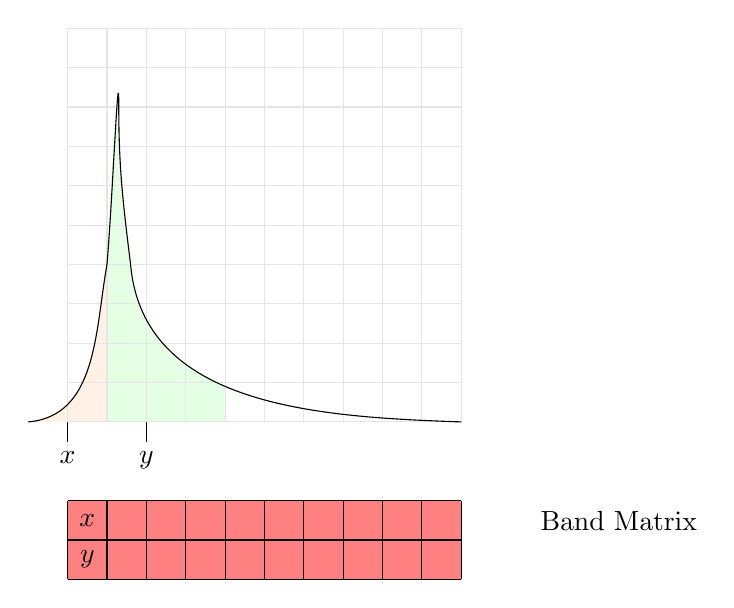
\begin{tikzpicture}
    
    \draw[gray!20] (0,-.5) -- (0,5);
    \draw[gray!20] (-.5,0) -- (5,0);
    \fill[fill=orange!10] (-.5,0) to [out=5,in=-100] (.5,2) to [out=85,in=90] (.5,0);
    \fill[fill=green!10] (.5,2) to [out=85,in=-100] (0.65,4) to [out=-90,in=97] (.8,2) to [out=-85,in=158] (2,.45) -- (2,0) -- (.5,0);

    \draw[gray!20] (0,0) grid[step=.5] (5,5);
    
    \draw [>=stealth] (-.5,0) to [out=5,in=-100] (.5,2) to [out=85,in=90] (0.65,4) to [out=-90,in=97] (.8,2) to [out=-85,in=178] (5,0);
    \fill[red!50] (0, -2) -- (5,-2) -- (5, -1) -- (0,-1);
    \draw (0,-2) grid[step=.5] (5,-1);
    \draw(7,-1.5) node[above] {Band Matrix};

    \draw(.25,-1.25) node {$x$};
    \draw(.25,-1.75) node {$y$};


    \draw (0,-.25) -- (0,0);
    \draw (1,-.25) -- (1,0);
    % \draw (2,-.25) -- (2,5);
    \draw(0,-.25) node[below] {$x$};
    \draw(1,-.25) node[below] {$y$};
    % \draw(2,-.25) node[below] {$N_{int}$};

 
\end{tikzpicture}


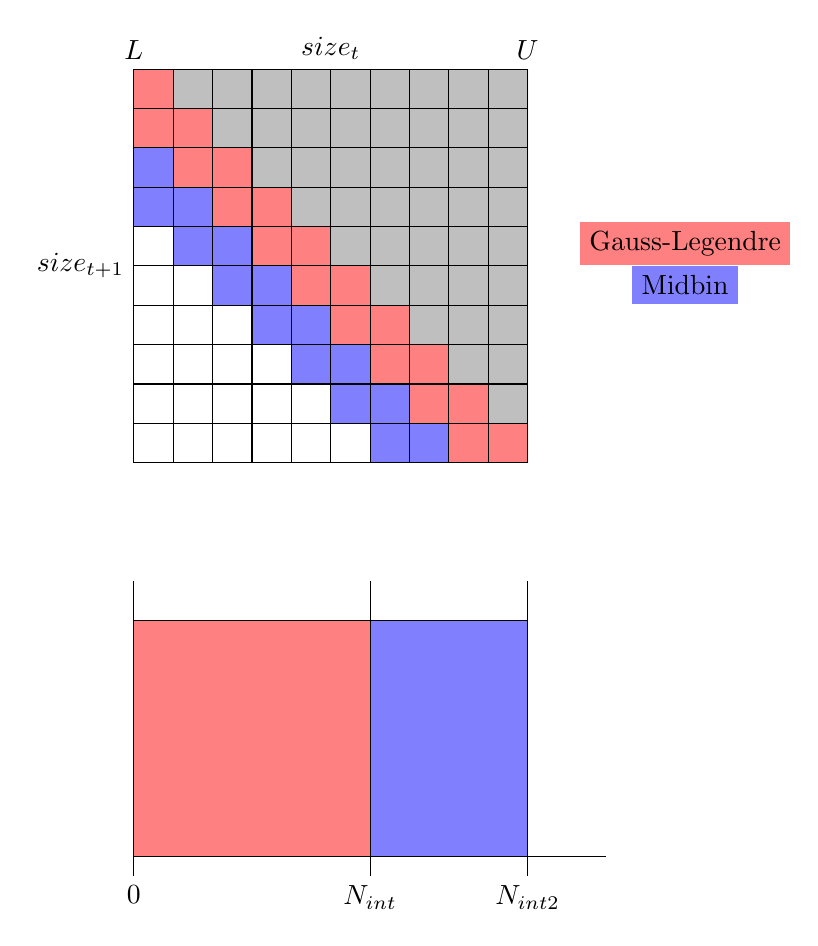
\begin{tikzpicture}
    \foreach \i in {3,2.5,...,0}{
            {\fill[blue!50] (\i, 5-\i-2) -- (5,5-\i-2) -- (5,5) -- (\i,5);}
    }
    \foreach \i in {4,3.5,...,0}{
            {\fill[red!50] (\i, 5-\i-1) -- (5,5-\i-1) -- (5,5) -- (\i,5);}
    }
    \foreach \i in {5,4.5,...,0.5}{
            {\fill[gray!50] (\i, 5-\i) -- (5,5-\i) -- (5,5) -- (\i,5);}
    }

    \draw (0,0) grid[step=.5] (5,5);
    \draw (2.5,5) node[above]{$size_t$} ;
    \draw (0,2.5) node[left]{$size_{t+1}$} ;
    \draw(0,5) node[above] {$L$};
    \draw(5,5) node[above] {$U$};

    \draw(7,2.5) node[fill=red!50,above] {Gauss-Legendre};
    \draw(7,2.5) node[fill=blue!50,below] {Midbin};

    \begin{scope}[shift={(0,-5)}]
    \fill[red!50,draw=black] (0,0) -- (0,3) -- (3,3) -- (3,0);
    \fill[blue!50,draw=black] (3,0) -- (3,3) -- (5,3) -- (5,0);
    \draw (5,-.25) -- (5,3.5);
    \draw (0,-.25) -- (0,3.5);
    \draw (3,-.25) -- (3,3.5);
    \draw (5,-.25) -- (5,3.5);
    \draw (0,0) -- (6,0);
    \draw(0,-.25) node[below] {$0$};
    \draw(3,-.25) node[below] {$N_{int}$};
    \draw(5,-.25) node[below] {$N_{int2}$};
    \end{scope}
   

\end{tikzpicture}

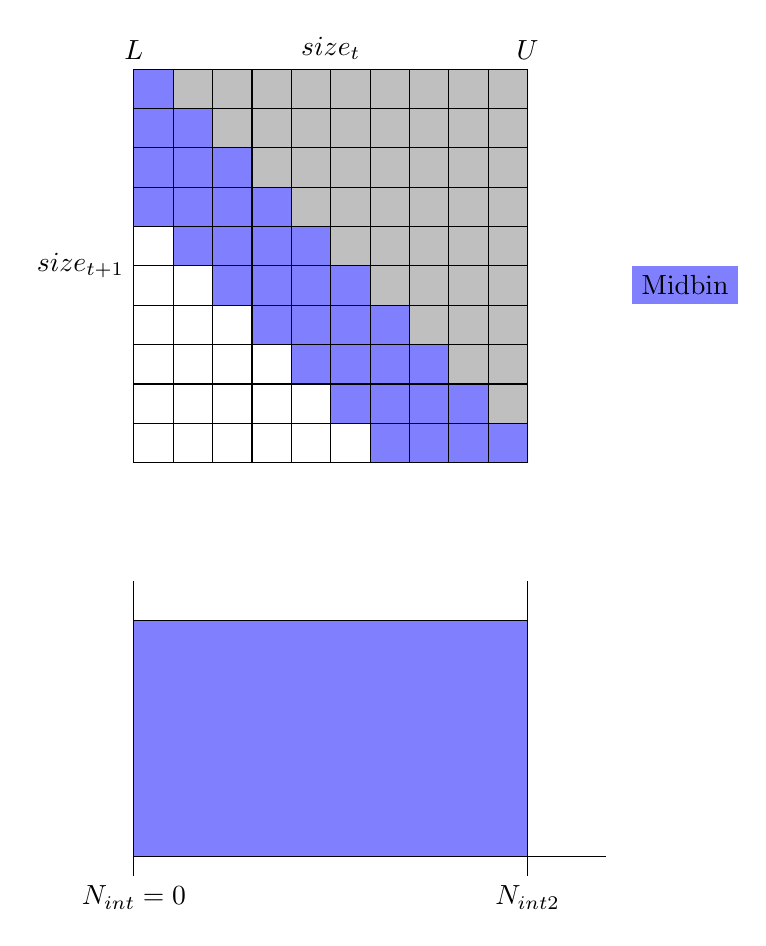
\begin{tikzpicture}
    \foreach \i in {3,2.5,...,0}{
            {\fill[blue!50] (\i, 5-\i-2) -- (5,5-\i-2) -- (5,5) -- (\i,5);}
    }
    \foreach \i in {5,4.5,...,0.5}{
            {\fill[gray!50] (\i, 5-\i) -- (5,5-\i) -- (5,5) -- (\i,5);}
    }

    \draw (0,0) grid[step=.5] (5,5);
    \draw (2.5,5) node[above]{$size_t$} ;
    \draw (0,2.5) node[left]{$size_{t+1}$} ;
    \draw(0,5) node[above] {$L$};
    \draw(5,5) node[above] {$U$};

    \draw(7,2.5) node[fill=blue!50,below] {Midbin};

    \begin{scope}[shift={(0,-5)}]
        \fill[blue!50,draw=black] (0,0) -- (0,3) -- (5,3) -- (5,0);
        \draw (5,-.25) -- (5,3.5);
        \draw (0,-.25) -- (0,3.5);
        \draw (5,-.25) -- (5,3.5);
        \draw (0,0) -- (6,0);
        \draw(0,-.25) node[below] {$N_{int} = 0$};
        \draw(5,-.25) node[below] {$N_{int2}$};
        \end{scope}

    

\end{tikzpicture}

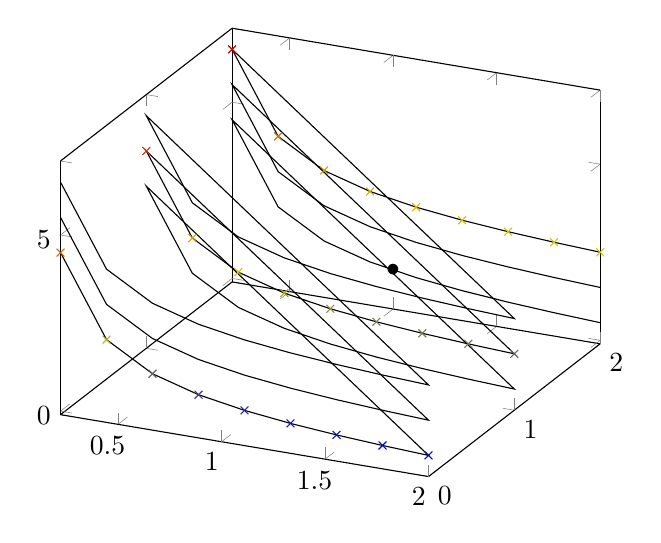
\begin{tikzpicture}
        \begin{axis}[]
\addplot3+ [domain=0:2, domain y = 0:2,samples = 10,
            samples y =3,only marks, scatter, mark = x] {1 /x + y};
        \foreach \l in {0,1,2}
            \addplot3 [domain=0:2,samples = 10,
            samples y =3] {1 /x + \l};

        \draw (1,2,1) node{$\bullet$};

%             \addplot3 [
%     domain=0:2,
%     domain y = -3:1,
%     samples = 20,
%     samples y = 8,
%     mesh] {1 /x + y};
% \addplot3+ [
%     domain=0:2,
%     domain y = 0,2,
%     samples = 10,
%     samples y = 3] {1/x+y};

        \end{axis}
        \end{tikzpicture}

\end{document}